% COMPILE: xelatex

\documentclass[a4paper]{article}  % A4 paper size

\usepackage[UTF8]{ctex}  % Chinese support
\usepackage[left=3.17cm, right=3.17cm, top=2.54cm, bottom=2.54cm]{geometry}  % Margins

\usepackage{xcolor}  % Color support
\usepackage{tcolorbox}  % Colored boxes

\usepackage{fancyhdr}  % Header and footer
\usepackage{graphicx, subcaption}  % Figures
\usepackage[shortlabels]{enumitem}  % Enumerate list
\usepackage[sort&compress]{gbt7714}  % Bibliography
\usepackage{hyperref}  % Hyperlinks
\usepackage{booktabs, array}  % Tables
\usepackage{multirow}  % Multirow
\usepackage{amsmath}  % Math

\tcbuselibrary{skins}  % Colored boxes
\tcbuselibrary{minted}  % Code blocks

\setmonofont[]{Fira Code}  % Monospaced font
\usemintedstyle{colorful}  % Code block style set up
\setenumerate{  % Enumerate list set up
    itemsep=0pt,
    partopsep=0pt,
    parsep=\parskip,
    topsep=0pt,
    itemindent=4em,
    leftmargin=0pt,
    listparindent=2em,
    label= (\arabic*)
}
\setitemize{  % Itemize list set up
    itemsep=0pt,
    partopsep=0pt,
    parsep=\parskip,
    topsep=5pt
}
\setdescription{  % Description list set up
    itemsep=0pt,
    partopsep=0pt,
    parsep=\parskip,
    topsep=5pt
}
\hypersetup{  % Hyperlinks set up
    unicode,
    colorlinks=true,
    linkcolor=black,
    urlcolor=black
}



\newtcblisting{codeblock}[2][]{
    listing engine=minted,
    boxrule=0.1mm,
    colback=white!98!black,
    colframe=white!80!black,
    listing only,
    left=5mm,
    enhanced,
    sharp corners=all,
    overlay={
        \begin{tcbclipinterior}
            \fill[white!98!black] (frame.south west) rectangle ([xshift=5mm]frame.north west);
        \end{tcbclipinterior}
    },
    minted language=#2,
    minted style=tango,
    minted options={fontsize=\small,breaklines,autogobble,linenos,numbersep=3mm,escapeinside=\#\#},#1  % Use \# as escape character
}


\begin{document}

\title{\textbf{语音合成}\\Matlab 大作业报告}  % Title
\author{陈子熠}
\date{\today}
\maketitle

\tableofcontents

\newpage

\section{语音预测模型}

\subsection{}\label{sec:1_1}

给定
\begin{align*}
    e(n) &= s(n) - a_1s(n-1) - a_2s(n-2) \\
\end{align*}

假设 $e(n)$ 是输入信号,$s(n)$ 是输出信号,等式两边同时取 Z 变换,得上述滤波器的传递函数:
\begin{align*}
    H(z) &= \frac{S(z)}{E(z)} = \frac{1}{1 - a_1z^{-1} - a_2z^{-2}}
\end{align*}

故 $b = 1$,$a = [1, -a_1, -a_2]$。

对于任意系统函数,每一对共轭极点对应一个衰减的正弦信号的特征响应。令该对共轭极点为 $\lvert{p\_i}\rvert e^{\pm j\Omega}$,幅角为 $\Omega$,则对应的共振峰频率为 $\Omega / 2\pi f$,其中 $f$ 为采样频率。

据此,可以计算出共振峰频率:
\begin{codeblock}{matlab}
function formants = sys_formant_cal(a, T)
    % Calculate the formant frequencies of a given system
    % a [array]: denominator coefficients of the system
    % T [float]: sampling period
    % return [array]: formant frequencies
    poles = roots(a);
    poles = poles(imag(poles) > 0);
    formants = sort(atan2(imag(poles), real(poles)) / (2 * pi * T));
end
\end{codeblock}

令 $a = [1, -a_1, -a_2]$,$T = 1/8000$,得到共振峰频率约为 $1000 Hz$。

用 zplane 绘制零极点图:
\begin{codeblock}{matlab}
    zplane(b, a);
\end{codeblock}
零极点图如图 \ref{fig:1_1_zplane}。可见,原点处有一二阶零点,右半平面单位圆内有两个共轭极点。
由此可知,该系统是一个带通滤波器,且系统稳定。

用 freqz 绘制频率响应:
\begin{codeblock}{matlab}
    freqz(b, a);
\end{codeblock}
频率响应如图 \ref{fig:1_1_freqz}。可见,确实是一个带通滤波器,且共振峰频率约为 $0.25\times\pi\ rad/sample$。在 8000 Hz 的采样频率下,即 $1000 Hz$,与理论计算相符。

用 impz 绘制单位样值响应:
\begin{codeblock}{matlab}
    impz(b, a, 200);
\end{codeblock}
单位样值响应如图 \ref{fig:1_1_impz}。

用 filter 绘制单位样值响应:
\begin{codeblock}{matlab}
i = [1, zeros(1, 199)];
o = filter(b, a, i);
figure;
stem(o);
xlabel('n (samples)');
ylabel('Amplitude');
title('Impulse Response of using Filter');
\end{codeblock}
单位样值响应如图 \ref{fig:1_1_impz_filter}。两种方式得到的单位样值响应一致。

\begin{figure}[ht]
    \centering
    \begin{subfigure}[b]{0.48\textwidth}
        \centering
        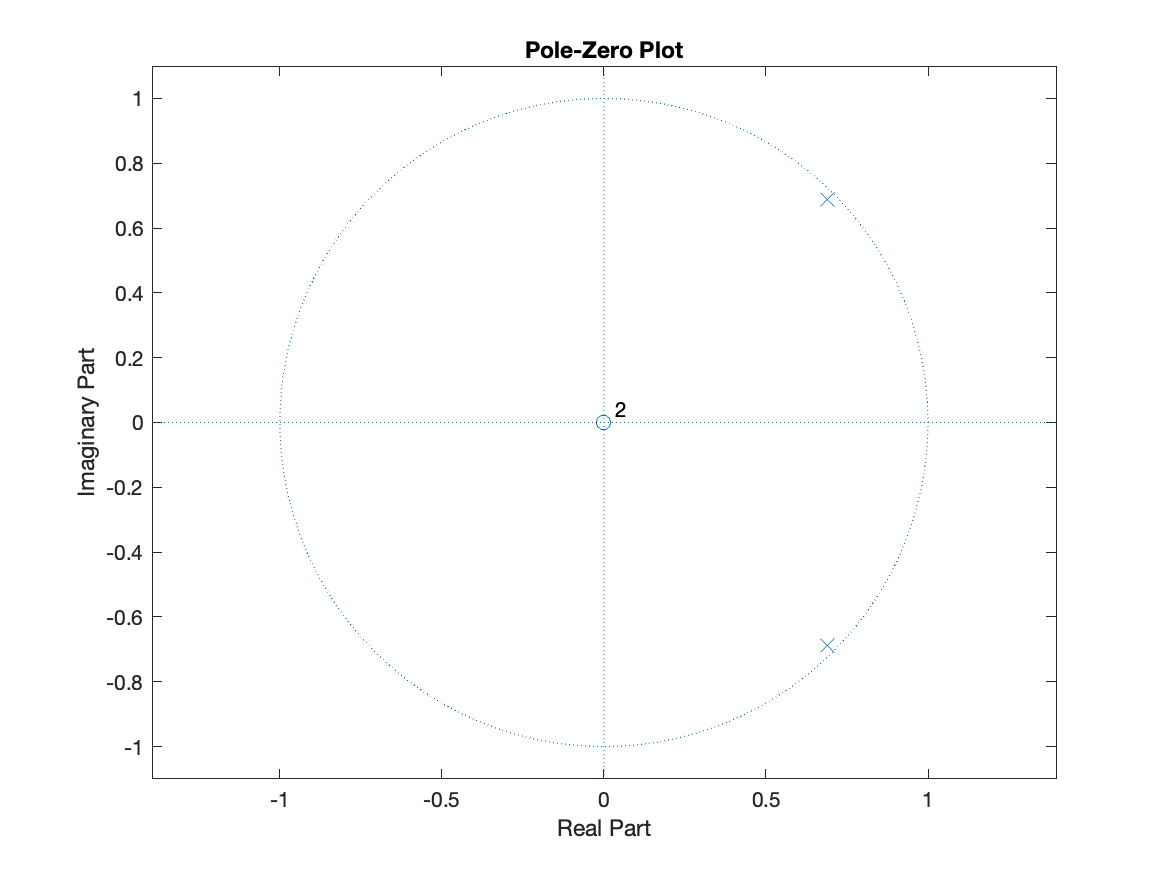
\includegraphics[width=\textwidth]{asserts/1_1_zplane.png}
        \caption{
            用 zplane 绘制的零极点图
        }\label{fig:1_1_zplane}
    \end{subfigure}
    \hfill
    \begin{subfigure}[b]{0.48\textwidth}
        \centering
        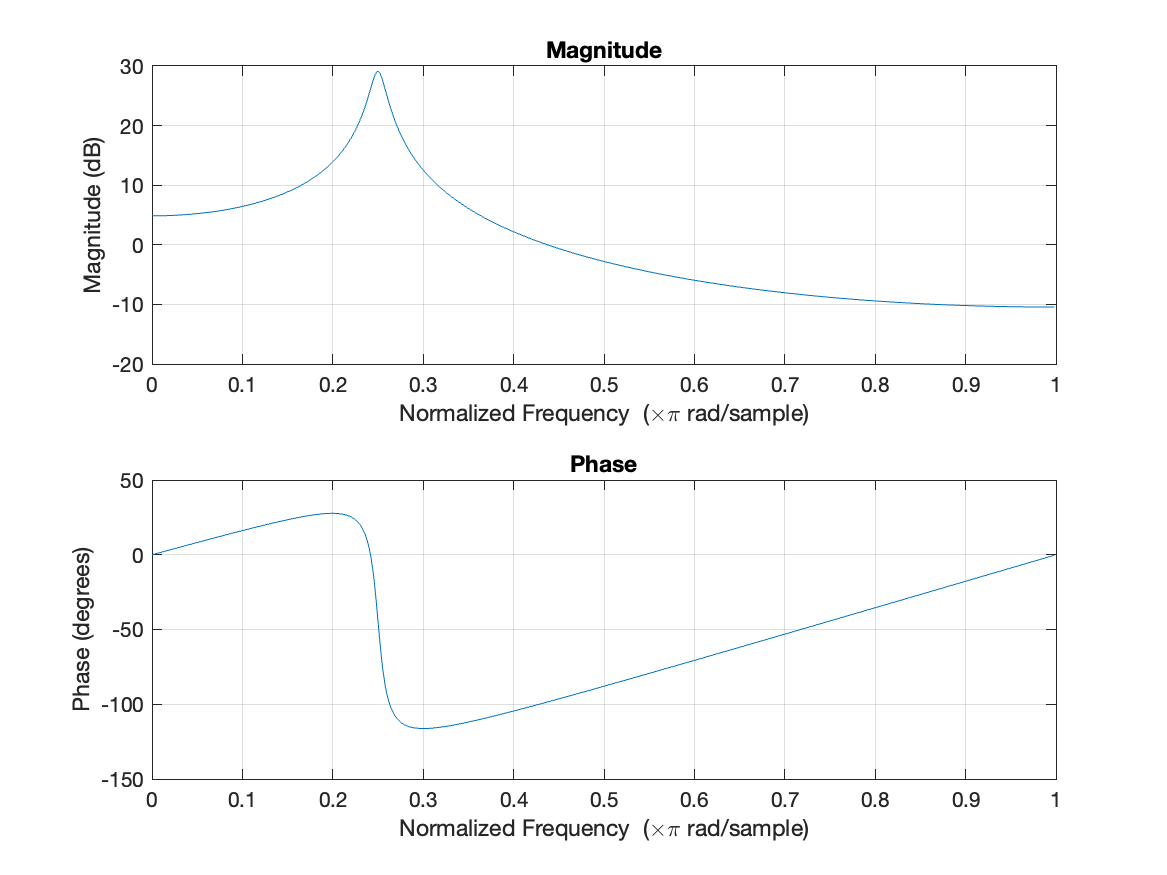
\includegraphics[width=\textwidth]{asserts/1_1_freqz.png}
        \caption{
            用 freqz 绘制的频率响应
        }\label{fig:1_1_freqz}
    \end{subfigure}
    \caption{
        零极点图与频率响应
    }
\end{figure}

\begin{figure}[ht]
    \begin{subfigure}[b]{0.48\textwidth}
        \centering
        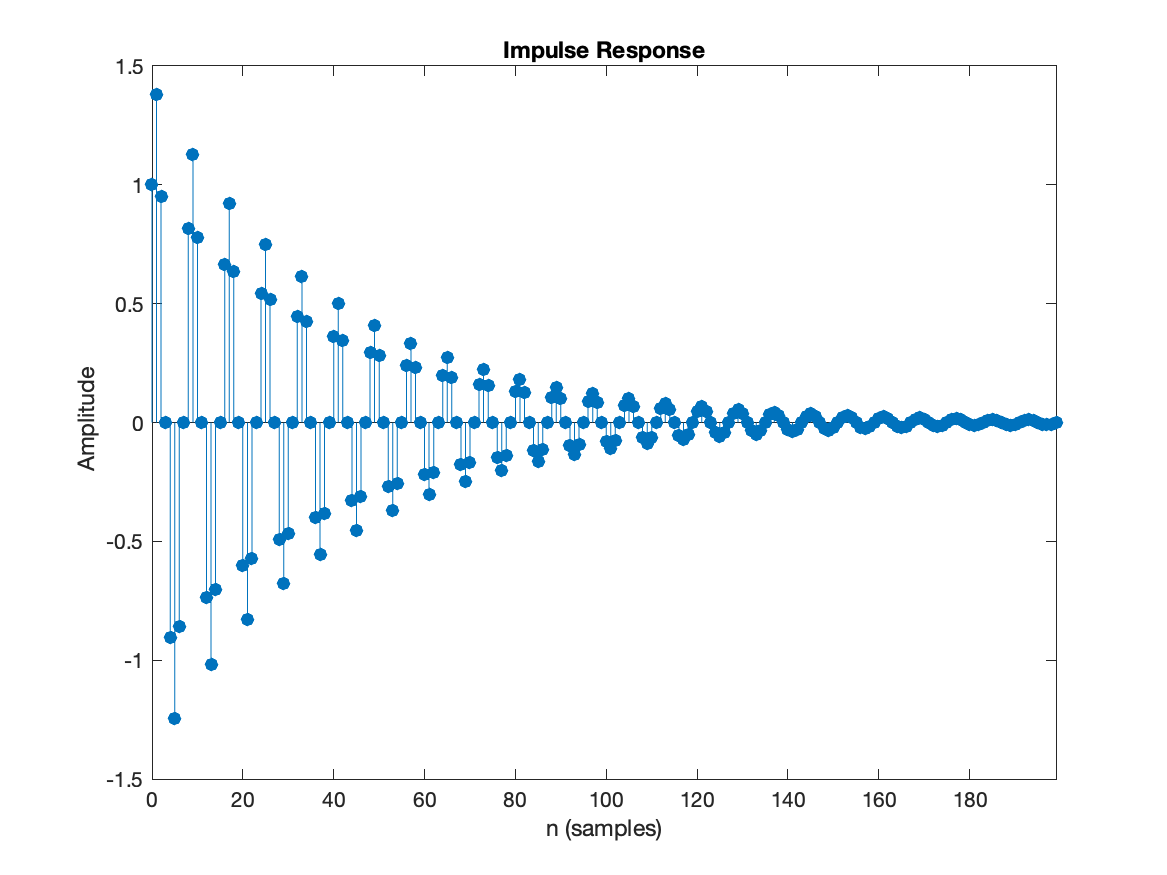
\includegraphics[width=\textwidth]{asserts/1_1_impz.png}
        \caption{
            用 impz 绘制的单位样值响应
        }\label{fig:1_1_impz}
    \end{subfigure}
    \hfill
    \begin{subfigure}[b]{0.48\textwidth}
        \centering
        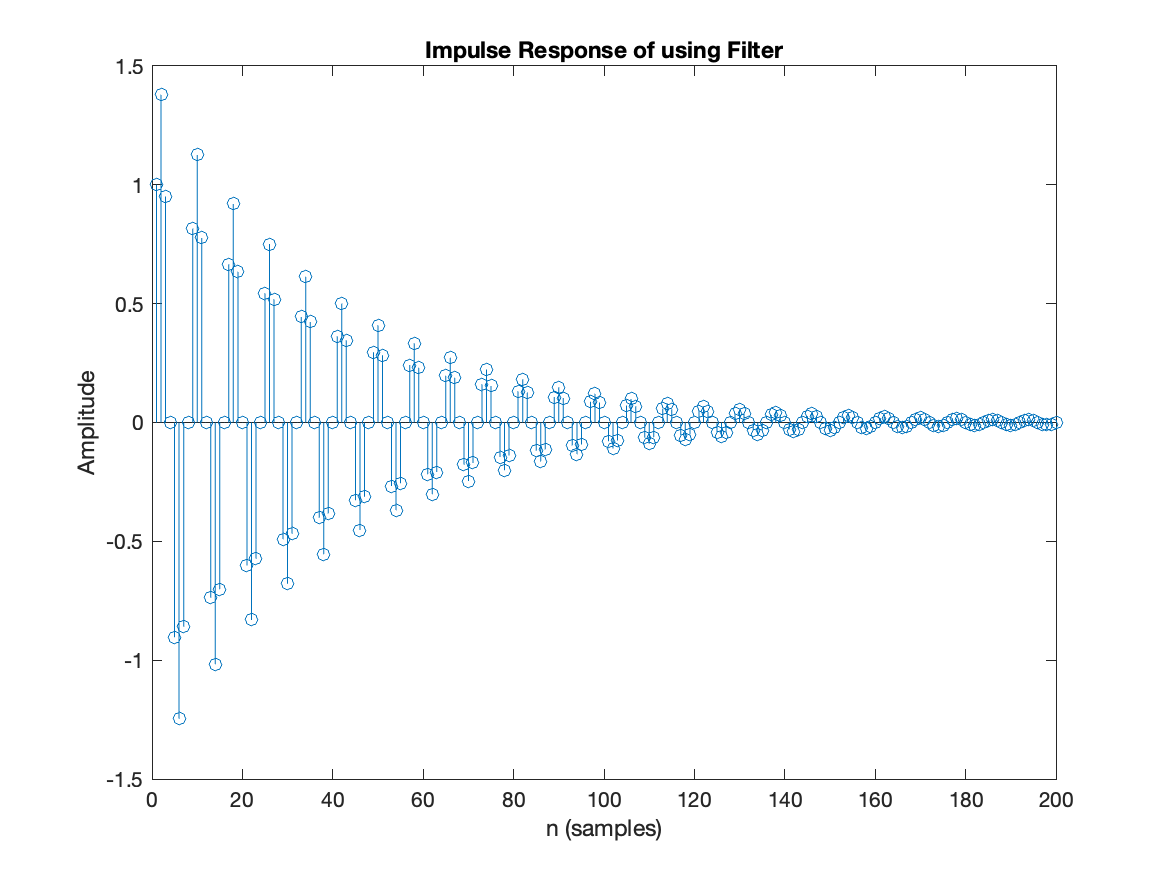
\includegraphics[width=\textwidth]{asserts/1_1_impz_filter.png}
        \caption{
            用 filter 绘制的单位样值响应
        }\label{fig:1_1_impz_filter}
    \end{subfigure}
    \caption{
        单位样值响应
    }
\end{figure}

\subsection{}

该程序的基本流程如下:
\begin{enumerate}[i]
    \item 定义帧长、窗口大小等参数。
    \item 加载音频文件,计算相关配置。
    \item 初始化合成的语音信号、合成滤波器的初始状态等。
    \item 依次处理每帧语音。首先用线性预测法计算系统系数,接着用 \texttt{filter} 函数根据系统函数计算激励,然后利用逆系统滤波重建语音信号。
    \item 同时,可以根据基音周期及合成激励的能量合成激励,并用合成激励和 \texttt{filter} 函数产生合成语音。
    \item 此外,还可以通过更改或保持基音周期、共振峰频率、合成激励的长度等参数,调整合成语音的速度、音调等特征。
    \item 在第 27 帧,观察预测系统的零极点图。
    \item 最后试听并画出所合成的语音,并保存文件。
\end{enumerate}

\subsection{}

第 27 帧时绘制预测系统的零极点图:
\begin{codeblock}{matlab}
if n == 27
    B = [1, zeros(1, P)];
    zplane(A, 1); 
end
\end{codeblock}

零极点图如图 \ref{fig:1_3_zplane}。可见,原点处有一十阶极点,单位圆内有 5 对共轭零点。
由于声道模型是预测模型的逆系统,因此其零极点图与预测模型的零极点图相反。

\begin{figure}[ht]
    \centering
    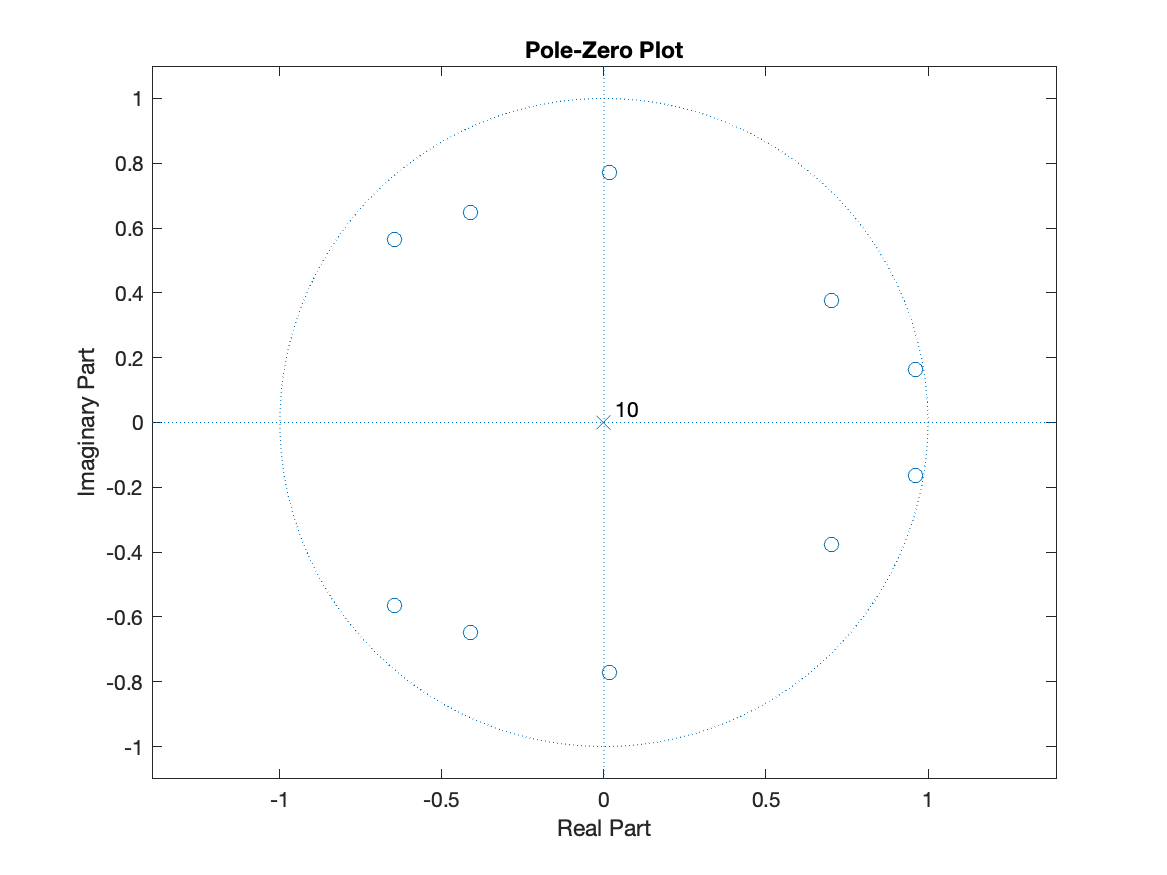
\includegraphics[width=.6\textwidth]{asserts/1_3_zplane.png}
    \caption{
        第 27 帧时预测系统的零极点图
    }\label{fig:1_3_zplane}
\end{figure}

\subsection{}

用 \texttt{filter} 计算激励信号:
\begin{codeblock}{matlab}
[exc((n - 1) * FL + 1 : n * FL), zi_pre] = filter(A, 1, s_f, zi_pre);
\end{codeblock}

注意到,这里记录了滤波器的状态,在下一帧作为初始状态使用,以保证连续性。

\subsection{}

用 \texttt{filter} 重建语音信号:
\begin{codeblock}{matlab}
[s_rec((n - 1) * FL + 1 : n * FL), zi_rec] = filter(1, A, exc((n - 1) * FL + 1 : n * FL), zi_rec);
\end{codeblock}

同样,这里记录了滤波器的状态,在下一帧作为初始状态使用,以保证连续性。
同时,重建系统是预测系统的逆系统,因此只需将 \texttt{filter} 的参数互换即可。

\subsection{}

试听程序:
\begin{codeblock}{matlab}
function sig_sound(s, fs)
    % Play the sound of the signal
    % s [array]: signal
    % fs [float]: sampling frequency
    sound(s / max(abs(s)), fs);
    pause(length(s) / fs);
end
\end{codeblock}

注意这里对信号进行了归一化处理,以保证播放时的音量合适,不超过最大音量。

通过运行 \texttt{sig\_sound([s; exc; s\_rec], 8000);},可以听到原始语音、合成激励、合成语音。
语音内容均为 “电灯比油灯进步多了”。其中,原始语音和合成语音的声音均清晰、自然,且无法区分。而合成激励的声音则音量较低,且有明显的噪音、颗粒感。

为研究三者的区别,定义了绘制波形的函数,该方法在后续的实验中也会经常使用。主要逻辑如下(省略了部分辅助功能,如保存或显示图片等):
\begin{codeblock}{matlab}
function sig_plot_t(ss, t, titles, save_prefix)
    % Plot the signals in time domain
    % ss [cell]: signals
    % t [array]: time
    % titles [cell]: titles of the signals
    % save_prefix [str][optional]: prefix of the saved images
    max_y = max(cellfun(@max, cellfun(@abs, ss, 'UniformOutput', false)));
    figure;
    for i = 1 : length(ss)
        subplot(length(ss), 1, i);
        plot(t, ss{i});
        title(titles{i});
        ylabel('Amplitude');
        ylim([-max_y, max_y]);
    end
    xlabel('Time (s)');
end
\end{codeblock}

同时,定义绘制频域的函数,该方法在后续的实验中也会经常使用。主要逻辑如下(省略了部分辅助功能,如保存或显示图片等):
\begin{codeblock}{matlab}
function sig_plot_f(SS, f_max, titles, save_prefix)
    % Plot the signals in frequency domain
    % SS [cell]: signals
    % f_max [int]: maximum frequency
    % titles [cell]: titles of the signals
    % save_prefix [str][optional]: prefix of the saved images
    figure;
    for i = 1 : length(SS)
        subplot(length(SS), 1, i);
        plot(abs(SS{i}(1 : f_max)));
        title(titles{i});
        ylabel('Magnitude');
    end
    xlabel('Frequency (Hz)');
end
\end{codeblock}

调用该函数如下(之后的调用不再重复给出):
\begin{codeblock}{matlab}
% plot the signals in time domain
t = [1 : L] / 8000;
titles = {'Original Signal', 'Excitation Signal', 'Reconstructed Signal'};
sig_plot_t({s, exc, s_rec}, t, titles, './report/asserts/1_6');
% plot clipped signals in time domain
start_s = 1000;
end_s = 1500;
s_clip = s(start_s : end_s);
exc_clip = exc(start_s : end_s);
s_rec_clip = s_rec(start_s : end_s);
t = [1 : (end_s - start_s + 1)] / 8000 + start_s / 8000;
titles = {'Original Signal (Clipped)', 'Excitation Signal (Clipped)', 'Reconstructed Signal (Clipped)'};
sig_plot_t({s_clip, exc_clip, s_rec_clip}, t, titles, './report/asserts/1_6_clipped');
% plot the signals in frequency domain
titles = {'Original Signal Spectrum', 'Excitation Signal Spectrum', 'Reconstructed Signal Spectrum'};
sig_plot_f({fft(s), fft(exc), fft(s_rec)}, 8000, titles, './report/asserts/1_6');
\end{codeblock}    

整体波形如图 \ref{fig:1_6_signal_t},局部波形如图 \ref{fig:1_6_clipped_signal_t},频谱如图 \ref{fig:1_6_signal_f}。

\begin{figure}[ht]
    \centering
    \begin{subfigure}[b]{0.48\textwidth}
        \centering
        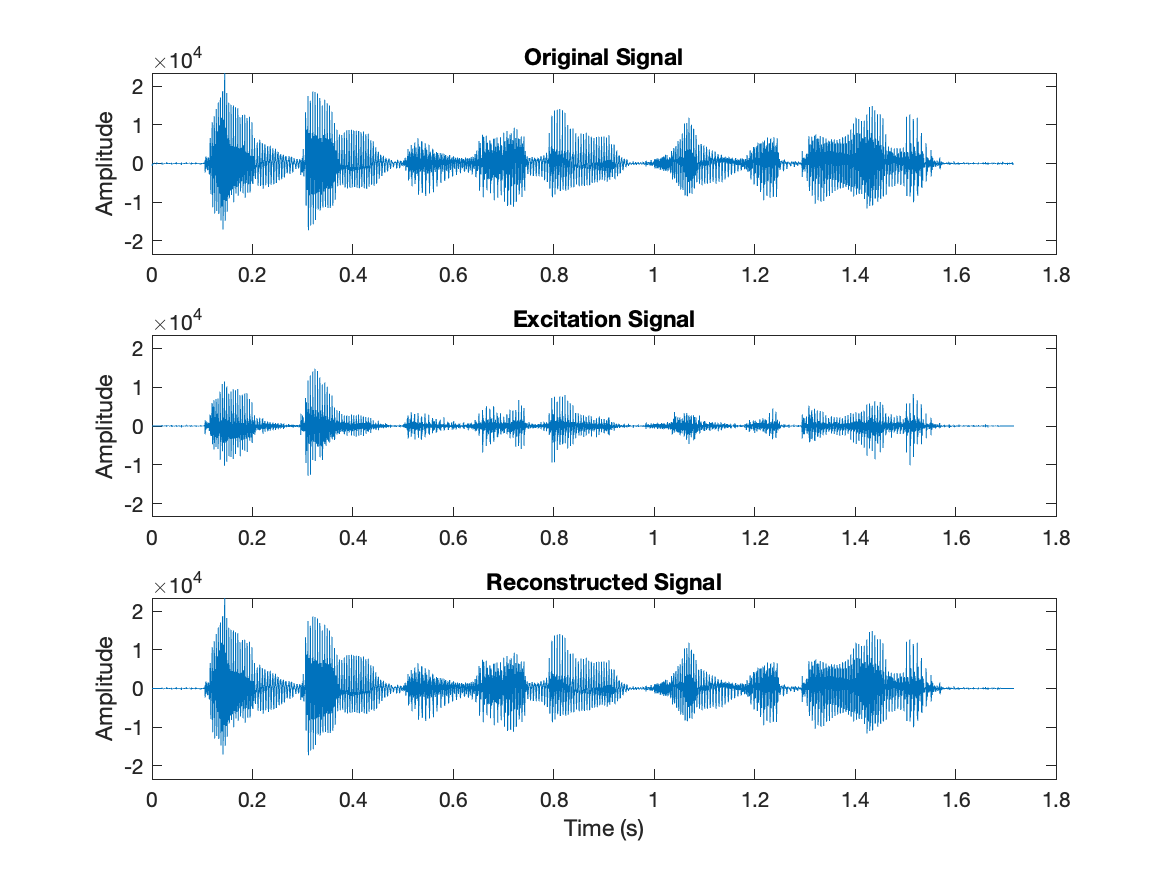
\includegraphics[width=\textwidth]{asserts/1_6_signal_t.png}
        \caption{
            整体波形
        }\label{fig:1_6_signal_t}
    \end{subfigure}
    \hfill
    \begin{subfigure}[b]{0.48\textwidth}
        \centering
        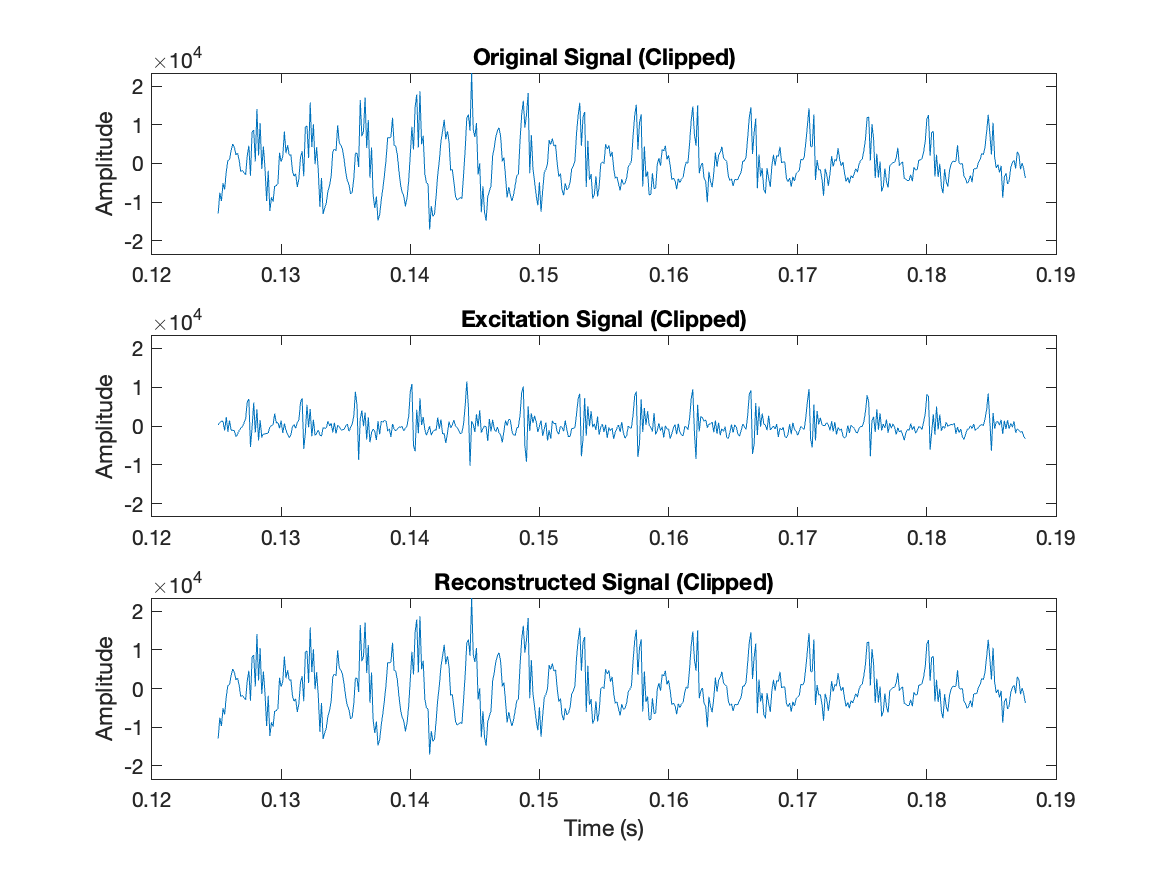
\includegraphics[width=\textwidth]{asserts/1_6_clipped_signal_t.png}
        \caption{
            局部波形
        }\label{fig:1_6_clipped_signal_t}
    \end{subfigure}
    \caption{
        原始语音、合成激励、合成语音波形
    }
\end{figure}

\begin{figure}[ht]
    \centering
    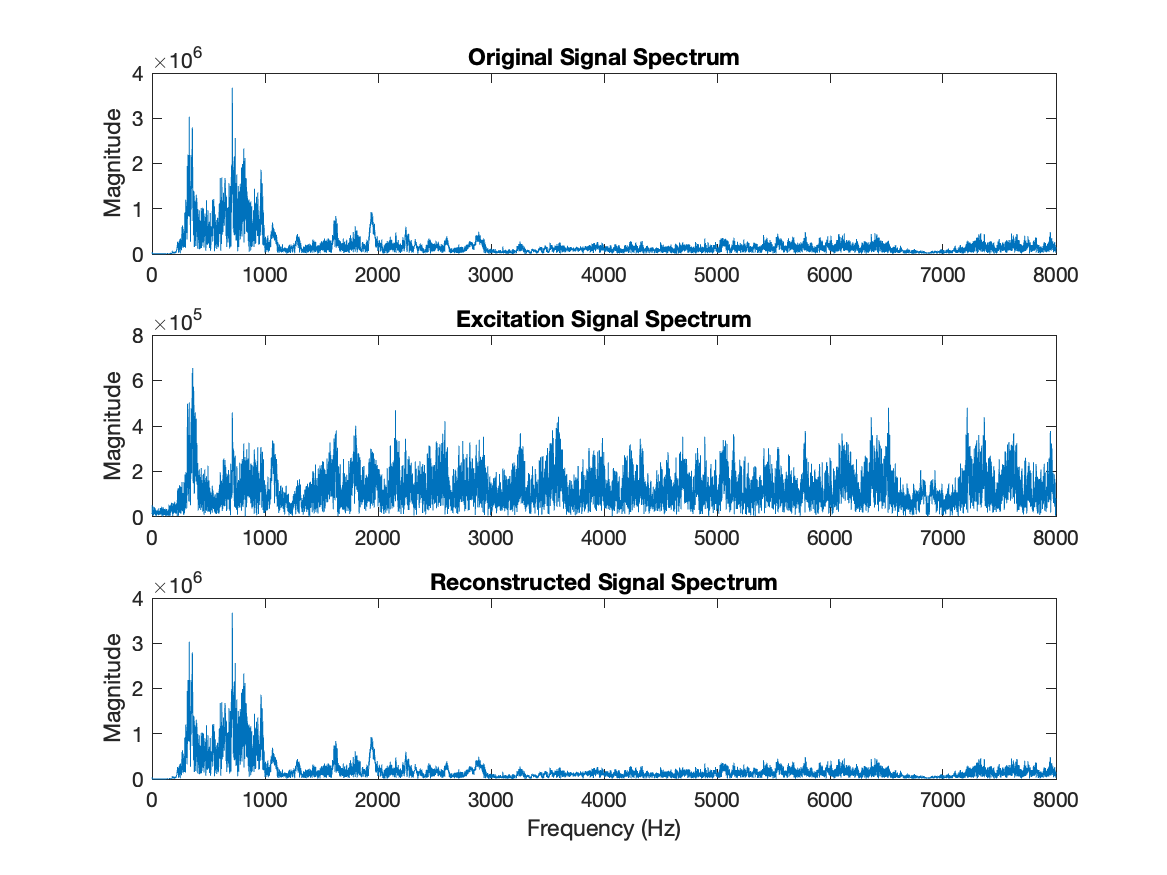
\includegraphics[width=.6\textwidth]{asserts/1_6_signal_f.png}
    \caption{
        原始语音、合成激励、合成语音频谱
    }\label{fig:1_6_signal_f}
\end{figure}

可见,原始语音、合成语音的波形和频谱基本一致,与听感一致。这是由于预测模型与重建模型互为逆系统,经过预测和重建后,语音信号能够保持不变。

而合成激励的波形和频谱则有明显差异。例如幅度较小、高频噪声较多,与听感一致。这表明在语音生成模型中,声门脉冲串含有丰富的谐波。


\section{语音合成模型}

\subsection{}

对单位样值串 $x(n) = \sum_{i=0}^{NS-1}\delta(n-iN)$,采样频率 $sr = 8000 Hz$,基音频率 $f_0 = 200 Hz$,则基音周期 $N = sr / f_0 = 40$。
若持续时间 $t = 1s$,则 $NS = f_0 \times t = 200$。

生成该基音周期固定的单位样值串,该方法在后续的实验中也会经常使用:
\begin{codeblock}{matlab}
function e = digit_sig_gen_const(PT, N)
    % Generate unit impulse signal
    % PT [int]: period
    % N [int]: length of the signal, including the zero padding
    % return [array]: unit impulse signal
    e = zeros(N, 1);
    e(1 : PT : N) = 1;
end
\end{codeblock}

生成并试听 200 Hz 和 300 Hz 的单位样值串:
\begin{codeblock}{matlab}
e200 = digit_sig_gen_const(8000 / 200, 8000);
e300 = digit_sig_gen_const(8000 / 300, 8000);
sig_sound([e200; e300], 8000);
\end{codeblock}

可以听到,300 Hz 的音调更高,约高半个八度。这与理论八度数 $\log_2(\frac{300}{200}) \approx 0.585$ 相符。

\subsection{}

利用循环生成基音周期按指定规律变化的单位样值串:
\begin{codeblock}{matlab}
function e = digit_sig_gen_addon(N, seg_N, func)
    % Generate unit impulse signal with variable period
    % N [int]: length of the signal, including the zero padding
    % seg_N [int]: length of each segment
    % func [function]: function to generate the period of each segment
    % return [array]: unit impulse signal with variable period
    e = zeros(N, 1);
    idx = 1;
    while idx <= N
        e(idx) = 1;
        seg_idx = floor(idx / seg_N);
        PT = func(seg_idx);
        idx = idx + PT;
    end 
end
\end{codeblock}

其中 \texttt{func} 指示了基音周期随段序号的变化规律,在本例中,$func = 80 + 5\text{mod}(seg\_idx, 50)$。

生成并试听基音周期按指定规律变化的单位样值串:
\begin{codeblock}{matlab}
e_addon = digit_sig_gen_addon(8000, 80, @(x) 80 + 5 * mod(x, 50));
sig_sound(e_addon, 8000);
\end{codeblock}

听上去音调的确是逐渐变化的,且变化规律符合预期。

\subsection{}

将此基音周期按指定规律变化的单位样值串作为合成激励,输入 \ref{sec:1_1} 中的滤波器:
\begin{codeblock}{matlab}
s_addon = filter(1, [1, -1.3789, 0.9506], e_addon);
sig_sound(s_addon, 8000);
\end{codeblock}

听上去,相比原信号,合成信号更沉闷,不再刺耳,类似通过一个管道发出的声音。

做出原信号、合成信号的波形和频谱如图 \ref{fig:1_9_signal_t} 和 \ref{fig:1_9_signal_f}。

可见,合成信号的波形变得更加平滑,与听感一致。同时,频谱在 1000 Hz 附近有明显的峰值,与预测模型的共振峰频率相符。同时,频谱以 4000 Hz 为对称轴,与离散信号频谱周期性的特点相符。

\begin{figure}[ht]
    \centering
    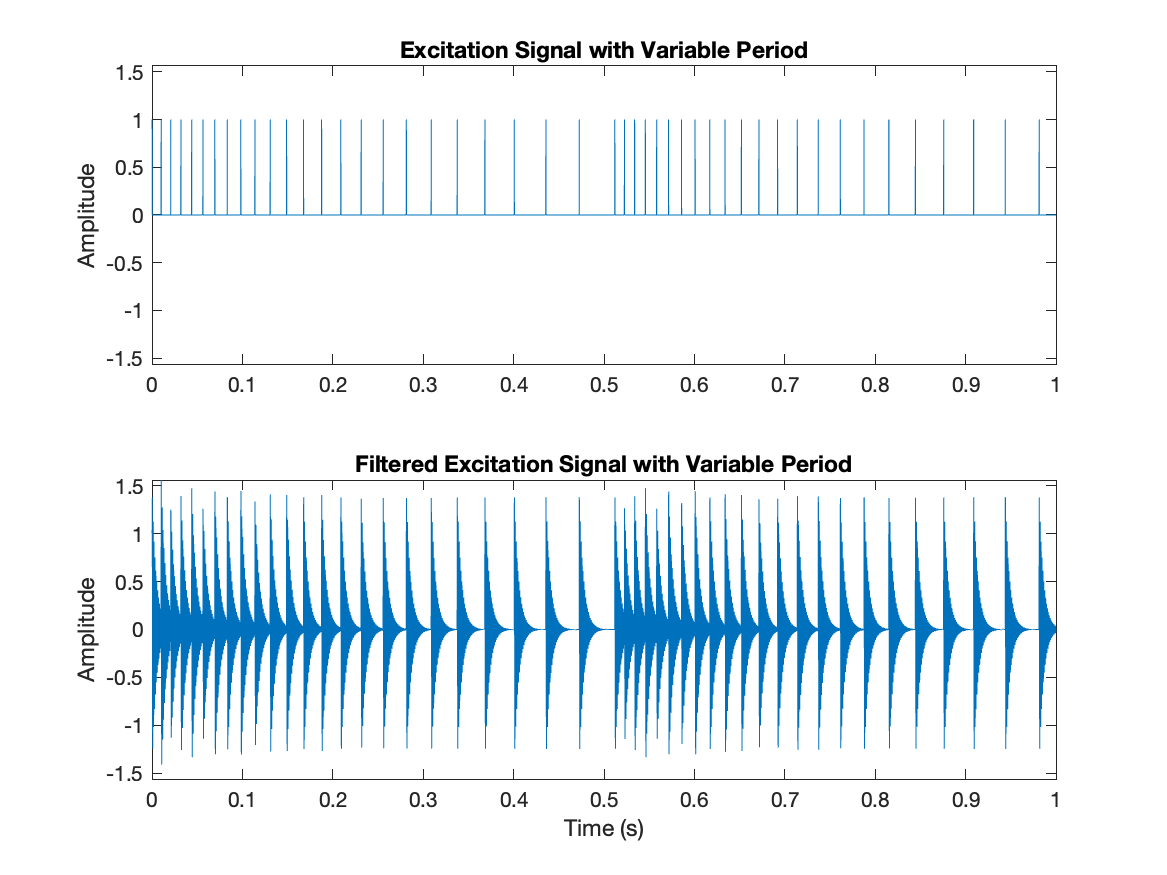
\includegraphics[width=.6\textwidth]{asserts/1_9_signal_t.png}
    \caption{
        原始语音、合成语音波形
    }\label{fig:1_9_signal_t}
\end{figure}

\begin{figure}[ht]
    \centering
    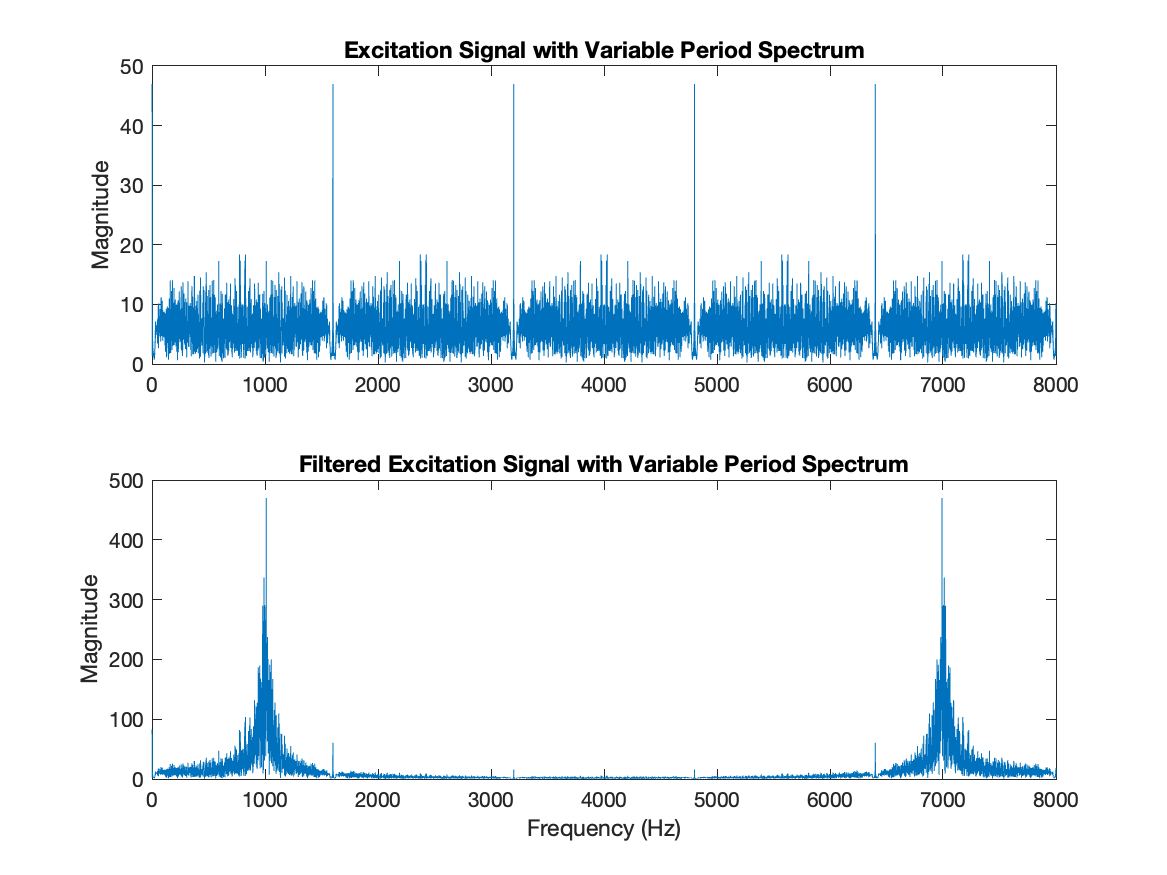
\includegraphics[width=.6\textwidth]{asserts/1_9_signal_f.png}
    \caption{
        原始语音、合成语音频谱
    }\label{fig:1_9_signal_f}
\end{figure}

\subsection{}

合成激励与语音:
\begin{codeblock}{matlab}
exc_syn((n - 1) * FL + 1 : n * FL) = G * digit_sig_gen_const(PT, FL);
[s_syn((n - 1) * FL + 1 : n * FL), zi_syn] = filter(1, A, exc_syn((n - 1) * FL + 1 : n * FL), zi_syn);
\end{codeblock}

其中,合成激励的基音周期为 \texttt{PT},合成语音的增益为 \texttt{G}。
\texttt{zi\_syn} 记录了滤波器的状态,在下一帧作为初始状态使用,以保证连续性。

试听并画出时域波形和频谱如图 \ref{fig:1_10_synthesized_signal_t} 和 \ref{fig:1_10_synthesized_signal_f}:

\begin{figure}[ht]
    \centering
    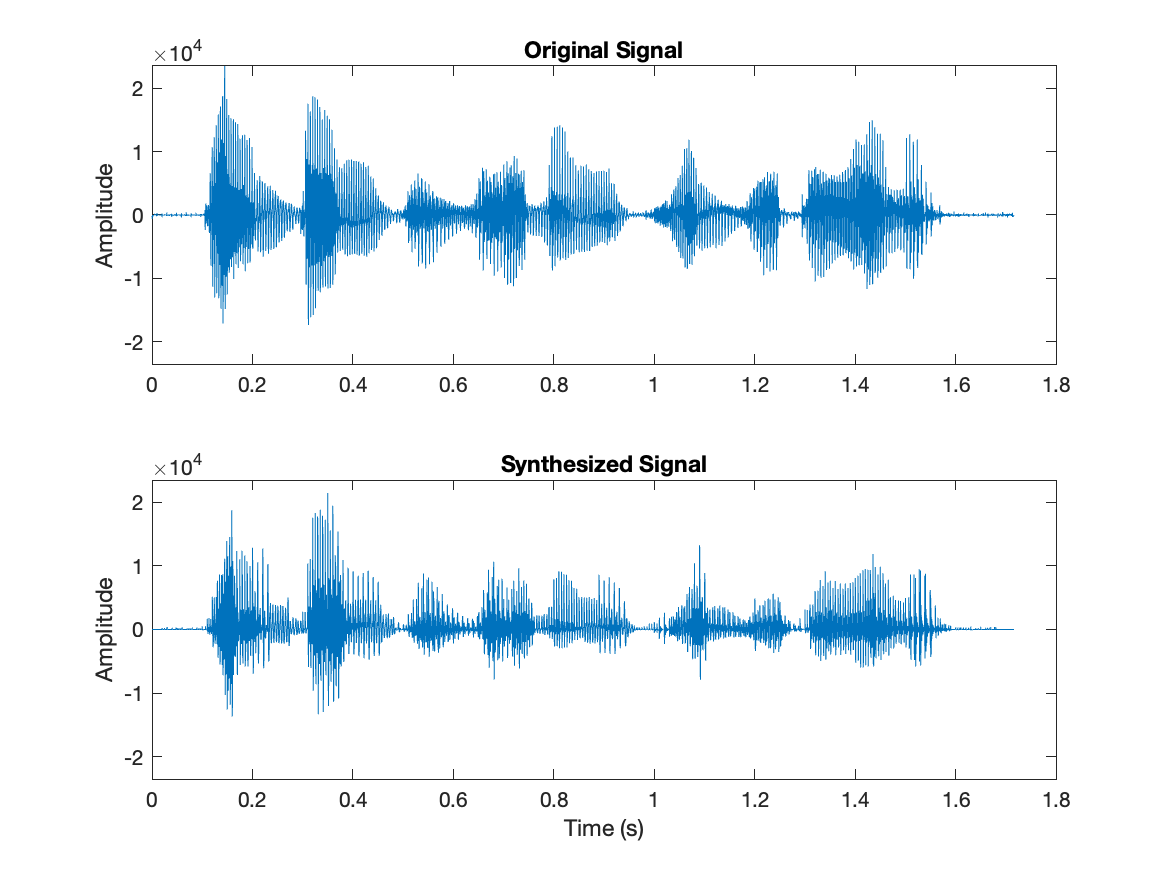
\includegraphics[width=.6\textwidth]{asserts/1_10_synthesized_signal_t.png}
    \caption{
        合成语音波形
    }\label{fig:1_10_synthesized_signal_t}
\end{figure}

\begin{figure}[ht]
    \centering
    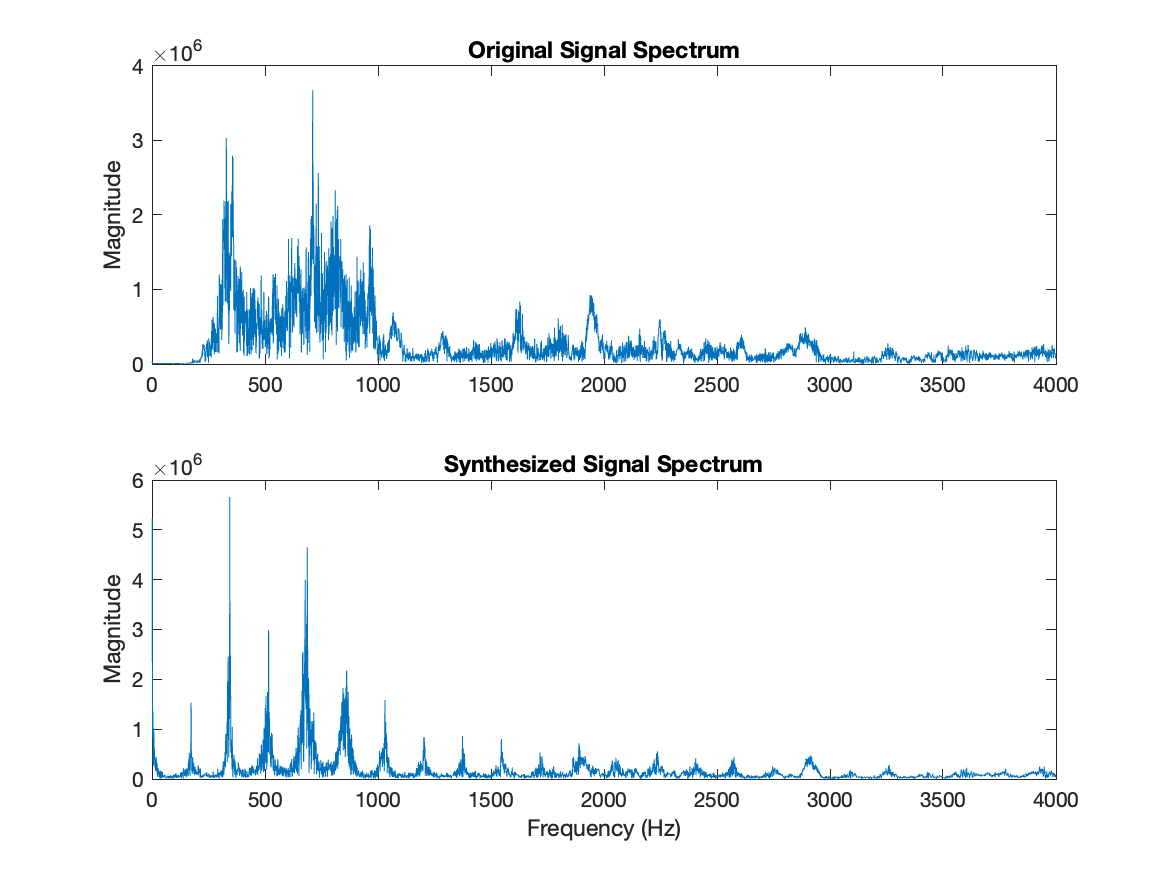
\includegraphics[width=.6\textwidth]{asserts/1_10_synthesized_signal_f.png}
    \caption{
        合成语音频谱
    }\label{fig:1_10_synthesized_signal_f}
\end{figure}

相比原信号,合成信号内容相近,音调、语速等特征也相近,但存在一定失真,颇有种机械合成的感觉。

波形上,两者变化趋势相仿,但并不完全相同,存在一定失真。频谱上,原信号的频率分量更丰富,而合成信号的频率分量更单一。

\section{变速不变调}

\subsection{}

激励的长度增加一倍,即帧长增加一倍 \texttt{FL\_v = 2 * FL}:
\begin{codeblock}{matlab}
exc_syn_v((n - 1) * FL_v + 1 : n * FL_v) = G * digit_sig_gen_const(PT, FL_v);
[s_syn_v((n - 1) * FL_v + 1 : n * FL_v), zi_syn_v] = filter(1, A, exc_syn_v((n - 1) * FL_v + 1 : n * FL_v), zi_syn_v);
\end{codeblock}

试听并画出时域波形和频谱如图 \ref{fig:1_11_speed_reduced_signal_t} 和 \ref{fig:1_11_speed_reduced_signal_f}:

\begin{figure}[ht]
    \centering
    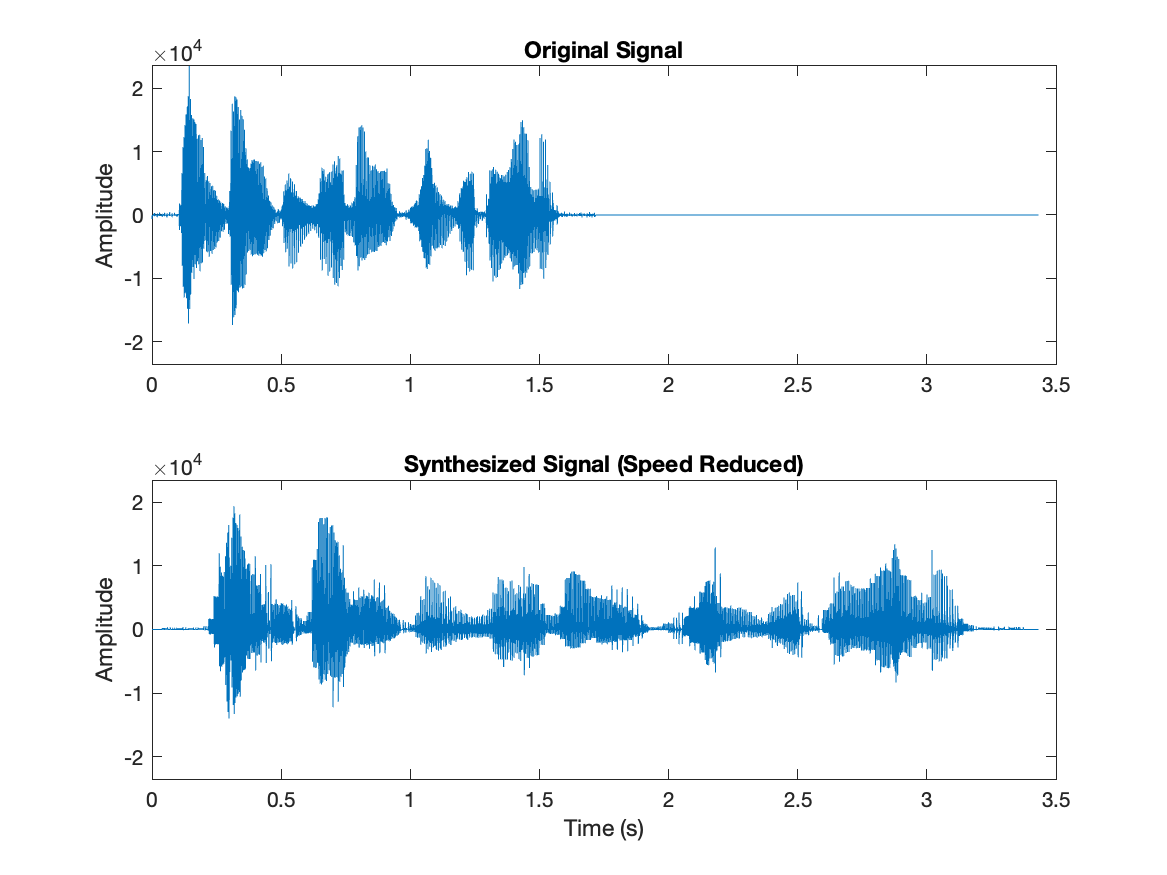
\includegraphics[width=.6\textwidth]{asserts/1_11_speed_reduced_signal_t.png}
    \caption{
        降速不变调合成语音波形
    }\label{fig:1_11_speed_reduced_signal_t}
\end{figure}

\begin{figure}[ht]
    \centering
    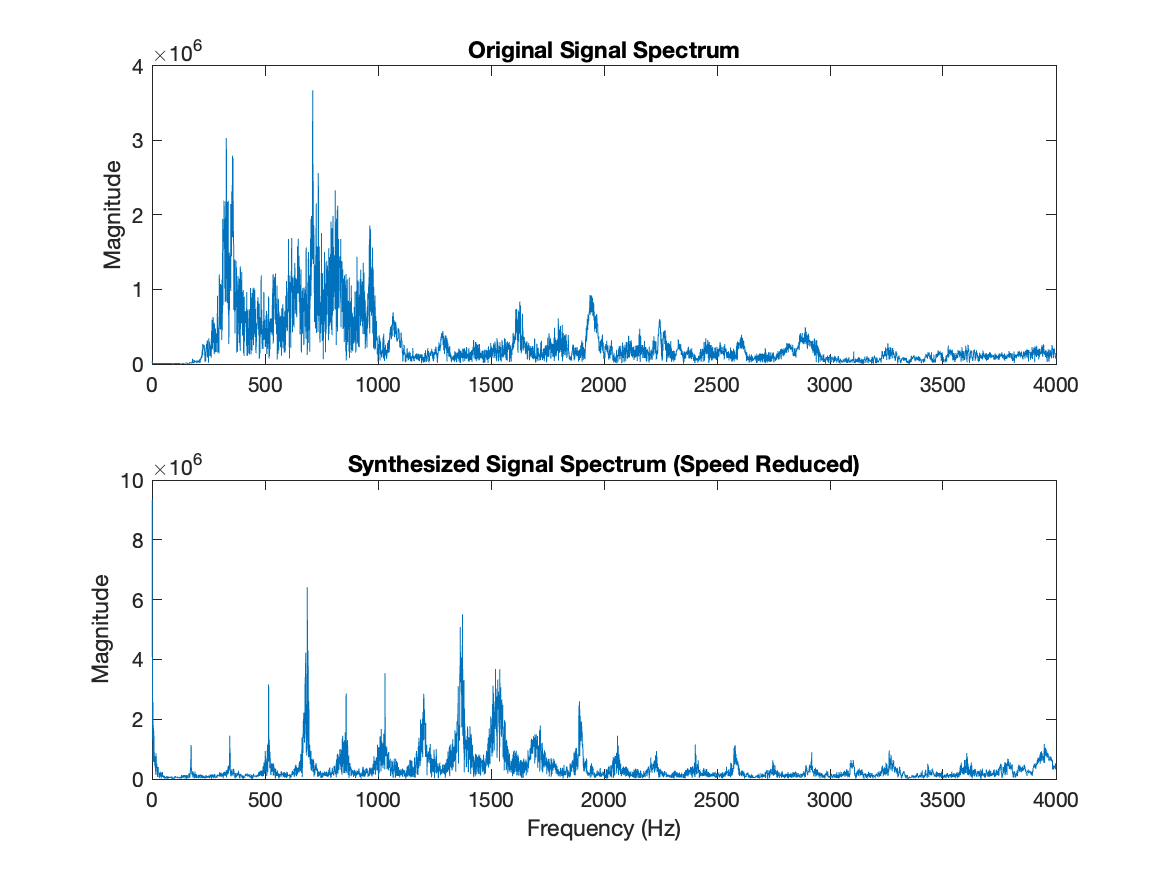
\includegraphics[width=.6\textwidth]{asserts/1_11_speed_reduced_signal_f.png}
    \caption{
        降速不变调合成语音频谱
    }\label{fig:1_11_speed_reduced_signal_f}
\end{figure}

相比原信号,降速不变调合成语音实现了变速不变调的效果,音调不变,语速变慢。

波形上,合成语音近似原信号在时间轴上拉长了一倍,与预期相符。频谱上,合成语音在更高的频率上出现了更多峰值,这是因为时间上的拉伸会导致频谱的压缩,但音调不变意味着基本频率和谐波结构应该保持不变。为了实现这一点,新的频谱成分需要分布在更宽的频率范围内,以保证原来的音调特征,补偿低频区域频谱的压缩效应。

\section{变调不变速}

\subsection{}

改变系统的共振峰频率:
\begin{codeblock}{matlab}
function rot_a = sys_rot_gen(a, angle)
    % Generate the rotated system
    % a [array]: denominator coefficients of the system
    % angle [float]: angle of rotation in radians
    % return [array]: denominator coefficients of the rotated system
    poles = roots(a);
    real_poles = poles(imag(poles) == 0);
    imag_poles = poles(imag(poles) > 0);
    imag_poles = imag_poles .* exp(1i * angle);
    all_poles = [imag_poles; conj(imag_poles); real_poles];
    rot_a = poly(all_poles) * a(1);
end
\end{codeblock}

这里将一、二象限的复极点按指定角度旋转,然后用 \texttt{poly} 函数生成新的系统系数。同时,保持实极点不变。

将 \ref{sec:1_1} 中的系统共振峰频率增加 150 Hz,相当于将一、二象限的复极点逆时针旋转 $\frac{150}{8000} \times 2\pi$:
\begin{codeblock}{matlab}
rot_A = sys_rot_gen(A, 150 * 2 * pi / 8000);
\end{codeblock}

做出该系统的频率响应如图 \ref{fig:1_12_freqz}。

\begin{figure}[ht]
    \centering
    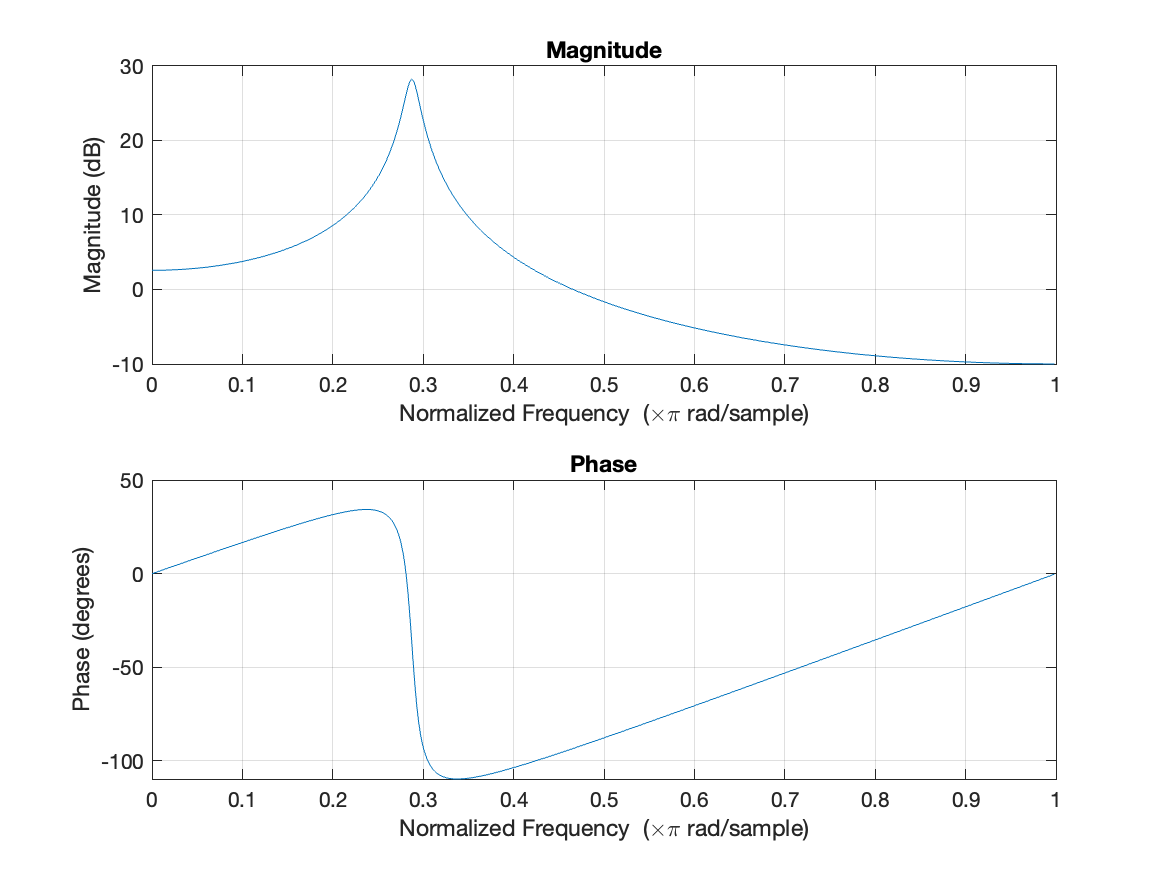
\includegraphics[width=.6\textwidth]{asserts/1_12_freqz.png}
    \caption{
        共振峰频率增加 150 Hz 的系统频率响应
    }\label{fig:1_12_freqz}
\end{figure}

可见,共振峰频率约为$0.2876\times \pi\ rad/sample$,即 1150 Hz,与预期相符。

\subsection{}

合成激励和语音:
\begin{codeblock}{matlab}
exc_syn_t((n - 1) * FL + 1 : n * FL) = G * digit_sig_gen_const(round(PT / 2), FL);
[s_syn_t((n - 1) * FL + 1 : n * FL), zi_syn_t] = filter(1, rot_A, exc_syn_t((n - 1) * FL + 1 : n * FL), zi_syn_t);
\end{codeblock}

其中,合成激励的基音周期为 \texttt{PT / 2},合成语音的增益为 \texttt{G},系统系数为 \texttt{rot\_A}。
\texttt{zi\_syn\_t} 记录了滤波器的状态,在下一帧作为初始状态使用,以保证连续性。

试听并画出时域波形和频谱如图 \ref{fig:1_13_pitch_increased_signal_t} 和 \ref{fig:1_13_pitch_increased_signal_f}:

\begin{figure}[ht]
    \centering
    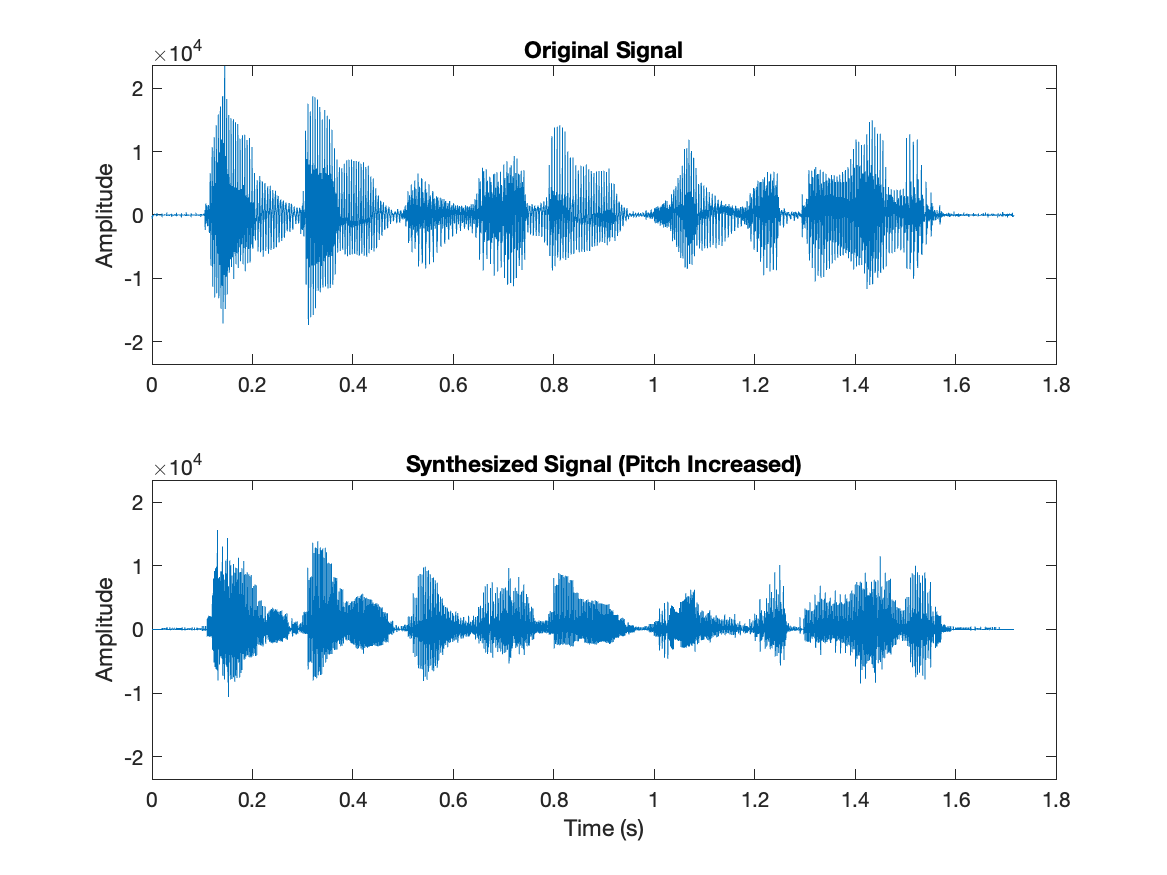
\includegraphics[width=.6\textwidth]{asserts/1_13_pitch_increased_signal_t.png}
    \caption{
        提升音调不变速合成语音波形
    }\label{fig:1_13_pitch_increased_signal_t}
\end{figure}

\begin{figure}[ht]
    \centering
    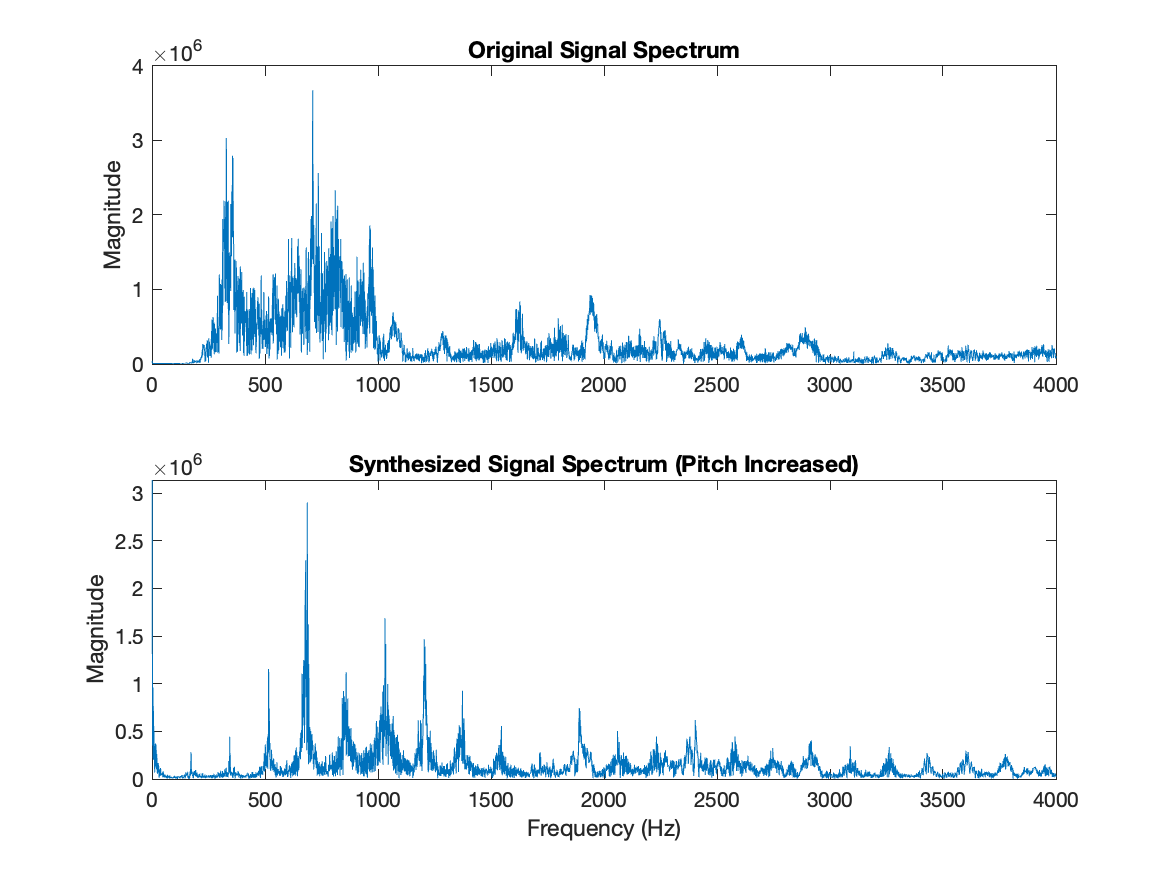
\includegraphics[width=.6\textwidth]{asserts/1_13_pitch_increased_signal_f.png}
    \caption{
        提升音调不变速合成语音频谱
    }\label{fig:1_13_pitch_increased_signal_f}
\end{figure}

相比原信号,提升音调不变速合成语音实现了变调不变速的效果,音调提升,语速不变。

波形上,合成语音变得更密集,但整体形状与原信号相似,与变调不变速的预期相符。频谱上,合成语音在更高的频率上出现了更多峰值,这印证了在音调提升的同时语速不变的现象。


\section{实验总结}

本次实验主要研究了语音合成的基本原理和方法,通过实现语音预测模型和语音合成模型,实现了语音的合成。在此基础上,进一步研究了变速不变调和变调不变速的方法,实现了这两种效果。

在实验中,我学会了如何用滤波器合成激励和语音,如何调整系统系数以实现变速不变调和变调不变速。同时,我学会了如何绘制波形和频谱图,如何试听合成语音,如何分析合成语音的特征。

除此以外,本次实验锻炼了我的 Matlab 编程能力,提高了我的信号处理和数字信号处理的实践能力。通过实验,我更加深入地理解了语音合成的原理和方法,对信号与系统的应用有了更深的认识。

\end{document}